\chapter[Session 3: Multithreading]{Multithreading}\label{chap:session3}
\chaptermark{Multithreading}
This lab session will dive into multithreading. In the previous assignments you learned the basics with regards to threads on a Linux system. In this assignment you will create a program that contains multiple threads. The objectives of this session are listed below:
	\begin{itemize}
		\item Learn the concept of multithreading
		\item Get to know the advantages and disadvantages of multitasking
	\end{itemize}

\section{Assignments}
A multithreaded process contains several different flows of control within the same address space. The benefits of multithreading include increased responsiveness to the user, resource sharing within the process, economy, and scalability factors, such as more efficient use of multiple processing cores. In the following assignments you have to write a program that consist of multiple threads. From these assignments it should become clear that threads are more easily to use than the regular processes. 

\subsection*{Assignment 3.1}
In the previous session you have learned how to create a single process. Processes can come in extremly handy but they suffer from a single point of failure. In this assignment you will get to know processes in a more advanced way, hoping to eludicate the advantages and disadvantages of multithreading processeses. You will use the LED extention board to visualy see what is going on. The objectives of this assignment are listed in the grey box below.
	\begin{objectives}
	    Objectives for a correct implementation of Assignment 3.1
	    
		Create a program (main function) that creates 3 threads. The program is only aloud to finish after the execution of all 3 threads! Lastly, you have to alter the output such that it outputs the currently active thread, it should correspond to the following structure: \code{[Thread?]:}. 
		
		\textbf{Thread 1 must implement:}
		\begin{itemize}[noitemsep]
			\item Blink the LED's with a certain self choosen pattern. This pattern could be whatever you want\\
		\end{itemize}
		
		\textbf{Thread 2 must implement:}
		\begin{itemize}[noitemsep]
			\item Count from 1 to 20 with 1 second in between each increment and print the updated counter value\\
		\end{itemize}
		
		\textbf{Thread 3 must implement:}
		\begin{itemize}[noitemsep]
			\item Create a 10x10 array with random numbers between 0 and 100 and print this array\\
		\end{itemize}
	\end{objectives}
	\signature 

\subsection*{Assignment 3.2}
In the previous assignment you created three processes that operated in a multithreaded regime. This assignment has the same method of approach. The difference lies in the difficulty of the assignment as this assignment will introduce binary counting! The objectives of this assignment are listed below.
    \begin{objectives}
    Objectives for a correct implementation of Assignment 3.2
    
        Use the source code of the previous assignment and alter it such that the output meets the following requirements. Keep in mind that you still have to output to currently active thread according to the same convention as mentioned in assignment 3.1
        
        \textbf{Thread 1 must implement:}
        \begin{itemize}
        \item Use the LED's on the extention board to make a binary counter which binary counts from zero to 10 and back to zero with 1 second in between each incremation. So for the value $5_{dec}$ the binary value is $0101_{bin}$ outputed and only LED's 1 and 3 should be active!
        \end{itemize}
        
        \textbf{Thread 2 must implement:}
        \begin{itemize}
        \item Make a counter from 10 to 0 and back to 10.
        \end{itemize}
        
        \textbf{Thread 3 must implement:}
        \begin{itemize}
        \item Rearrange the array created in the previous assignment in such a way the first column has ascending numbers\\
        \end{itemize}
    \end{objectives}
\signature
    
\subsection*{Assignment 3.3}
Write a multithreaded program that calculates various statistical values for a list of numbers. This program will be passed a series of numbers on the command line and will then create three separate worker threads. One thread will determine the average of the numbers, the second will determine the maximum value, and the third will determine the minimum value. For example, suppose your program is passed the integers:
\begin{flushleft}
	\code{90 81 78 95 79 72 85}
\end{flushleft}
 The program will report:
The average value is 82
The minimum value is 72 
The maximum value is 95

The objectives of this assignment are listed below
\begin{objectives}
Objectives for a correct implementation of Assignment 3.3

\begin{itemize}
\item The program must be able to listen to input values (sanitize the input to check if it is valid!)
\item Compute the average value
\item Compute the minimum value
\item Compute the maximum value
\item Compute the median value
\item Compute the standard deviation
\item Determine how many threads you should be using to assure a fast execution of the program.
\end{itemize}
\end{objectives}
\signature

\section{Bonus Question: Multithreaded Sorting Application}
Write a multithreaded sorting program that works as follows: A list of integers is divided into two smaller lists of equal size. Two separate threads (which we will term \textbf{sorting threads}) sort each sublist using a sorting algorithm of your choice. The two sublists are then merged by a third thread — a \textbf{merging thread} — which merges the two sublists into a single sorted list.

\begin{figure}[hbp]
\centering
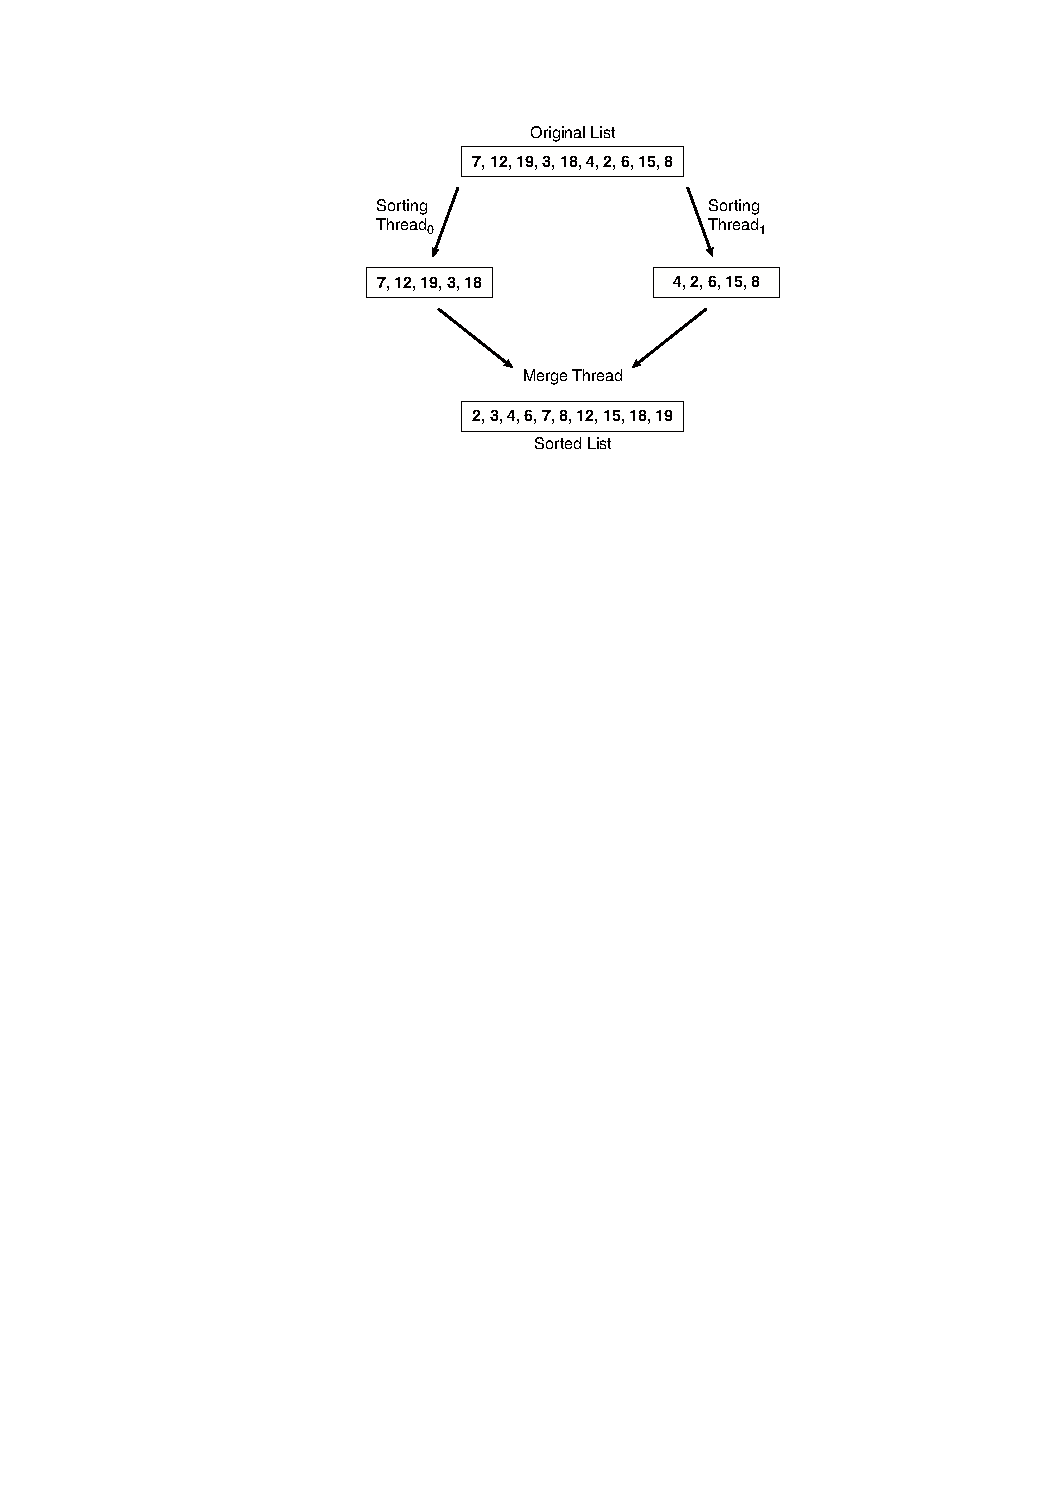
\includegraphics[width=0.5\textwidth]{images/multisort.pdf}
\caption{Multithreaded Sorting}
\label{fig:multi}
\end{figure}

Because global data are shared cross all threads, perhaps the easiest way to set up the data is to create a global array. Each sorting thread will work on one half of this array. A second global array of the same size as the unsorted integer array will also be established. The merging thread will then merge the two sublists into this second array. Graphically, this program is structured according to Figure \ref{multi}.
This programming project will require passing parameters to each of the sorting threads. In particular, it will be necessary to identify the starting index from which each thread is to begin sorting. Refer to the instructions of section \ref{sec:sudoku} for details on passing parameters to a thread. The parent thread will output the sorted array once all sorting threads have exited.\\
\signature

